\chapter{\textit{Git}}

\textit{Git} is a distributed version-control system for tracking changes in source code during the software development, and it can be used on cross platforms including Windows, Unix/Linux and MacOS. This section introduces the basic use of \textit{Git} on a local Linux machine and on a remote host such as \textit{GitHub}. Some contents in this section is taken from an earlier article \textit{A Git Tutorial}.

\section{Brief Introduction to \textit{Git}}

\textit{Git}, created by Linus Trovalds in 2005, is a distributed version-control system for tracking changes in source code and files. It is helpful with maintaining data integrity during the collaborative development of a software in distributed non-linear work flows. \textit{Git} is free and open-source software under GNU general public license.

With \textit{Git}, all computers participating in the software development store a copy of the full-fledged repository locally with complete history, and it can synchronize with a centralized remote server. \textit{Git} uses ``master'' and ``slave'' branches to manage the concurrent development of different features of the project, where the ``master branch'' is the stable and shared repository among everyone, and the ``slave branches'' are copies of the master branch where individual features can be developed. For a slave branch, once its developed feature is approved, it can be merged back to the master branch. A demonstration is given in Fig. \ref{ch:sma:fig:gitflow}.
\begin{figure}[htbp]
	\centering
	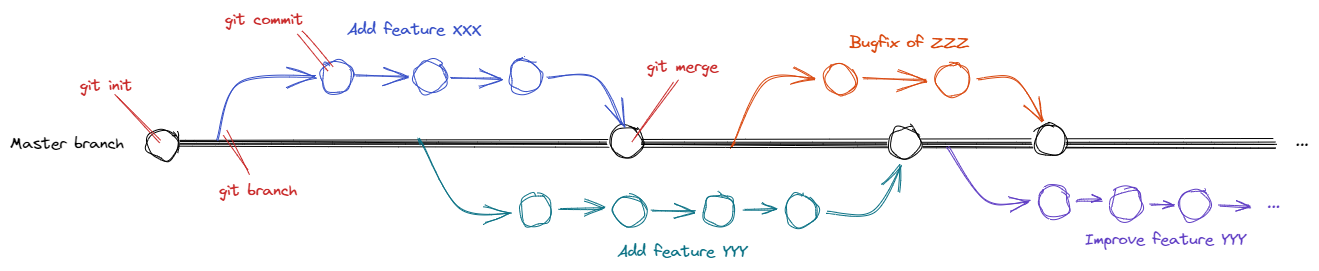
\includegraphics[width=350pt]{chapters/ch-software-management-advanced/figures/gitflow.png}
	\caption{\textit{Git} for software development management.} \label{ch:sma:fig:gitflow}
\end{figure}

CLI is often used to manage a \textit{Git} repository. For example, \verb|git init| starts a new repository with an empty master branch, and \verb|git branch <branch-name>| creates a new slave branch from the master branch, etc. Some of these commands are shown in Fig. \ref{ch:sma:fig:gitflow} and more details are introduced later. Notice that a graphical user interface is also available to interact with \verb|git|. However, in the scope of this notebook, command line is mostly used.

\section{Initial Setup}

To use \textit{Git}, follow the instructions to install and configure the software.

\subsection{Installation}

\textit{Git} and its relevant documents can be obtained from its official website \textit{https://git-scm.com/}. In many Linux distributions, \textit{Git} is pre-installed. If \textit{Git} is missing in the machine, follow the instructions on the official website to install it on the computer. Notice that the installation procedure may differ according to the OS.

\subsection{Configuration}

Upon successful installation, it is recommended to use \verb|git config| for some basic configurations. Notice that there are two types of configurations, namely the global configurations (apply to the machine and the user), and the repository configurations (apply to a particular \textit{Git} repository). By default, the global level configurations are stored under \verb|~/.gitconfig| and the repository level configurations \verb|./.git/config| in the repository. A good practice to edit these configurations is to use \textit{Git} commands rather than editing the files directly.

To add user name and email to the global configuration, use
\begin{lstlisting}
$ git config --global user.name '<user name>'
$ git config --global user.email '<user email>'
\end{lstlisting}
To retrieve the global configuration, use either \verb|git config --global -l| or \verb|cat ~/.gitconfig|. To revoke a global configuration, use
\begin{lstlisting}
$ git config --global --unset <configuration>
\end{lstlisting}
For example,
\begin{lstlisting}
$ git config --global --unset user.name
\end{lstlisting}
removes the user name.

More details about \verb|git config| can be found at \textit{https://git-scm.com/docs/git-config}. Usually, the user name and email configurations are mandatory, as they are very useful information in developing collaborative projects.

\section{Local Repository Management}

\textit{Git} can be used to manage a purely local repository. Although this is not its full power, \textit{Git} is still useful. In this scenario, \textit{Git} is most often used to track versions and control branches (when the developer wants a dedicate branch for a adding a new feature).

\subsection{Initialization of Repository}

Navigate to the project directory. Use the following command to create a new \textit{Git} repository for the project.
\begin{lstlisting}
$ git init
\end{lstlisting}
From this point forward, \textit{Git} monitors everything that happens inside this directory and its subdirectories and tries to track any change to the files, unless otherwise configured specifically. A bench of \textit{Git} commands is enabled, such as \verb|git status| that checks the status of the repository.

\subsection{Version Tracking}

For simplicity, assume that there is only one branch in the repository, namely the master branch. Notice that when there are multiple branches, the version-tracking works the same for each and every branch in a separate and independent manner.

The mechanism behind version tracking is briefly introduced as follows. This helps the user to better understand how \textit{Git} works and how the CLI commands are designed.

The project directory is split into two parts, outside \verb|./.git/| the workspace, and inside \verb|./.git/| the \textit{Git} repository. The workspace has the up-to-date project contents and it is directly managed by the user, while \textit{Git} repository is managed by \textit{Git} and it is supposed to be invisible to the user unless interacted with the CLI.

Inside the \textit{Git} repository are metadata of the workspace files such as which files have been changed since the last deployment, etc. It also stores a full back up of every historical versions for the project (with powerful compressing mechanisms, of course). It is worth mentioning that instead of recording the changes of a file from version to version, \textit{Git} records the snapshot of the file in every version, unless it is left untouched between two consecutive versions.

Figure \ref{ch:sma:fig:gitbasics} gives a demonstration of how \textit{Git} manages the project directory. \textit{Git} classifies files in the workspace into different status, as shown in Fig. \ref{ch:sma:fig:gitbasics}. A brief explanation of each types is given in Table \ref{ch:sma:tab:gitbasics}. Detail explanations of ``stage'' and ``commit'' are given later.
\begin{figure}[htbp]
	\centering
	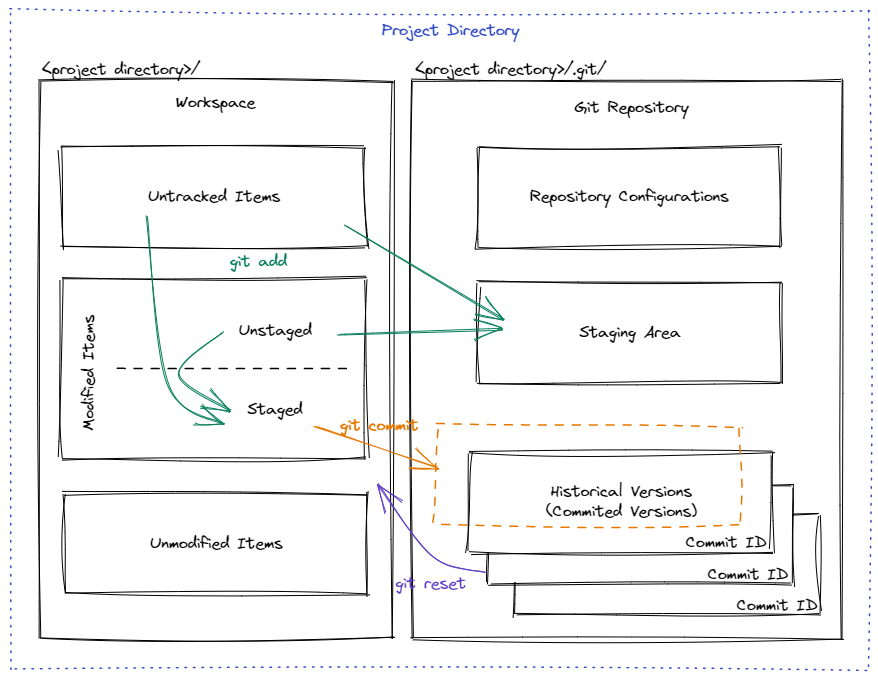
\includegraphics[width=350pt]{chapters/ch-software-management-advanced/figures/gitbasics.png}
	\caption{The project directory managed by \textit{Git}.} \label{ch:sma:fig:gitbasics}
\end{figure}

\begin{table}
	\centering \caption{Different file status in a \textit{Git} managed project.}\label{ch:sma:tab:gitbasics}
	\begin{tabularx}{\textwidth}{lX}
		\hline
		Status & Description \\ \hline
		Untracked & Newly added or renamed items in the project directory.  \\ \hdashline
		Modified (Unstaged) & Modified items from the last version that has not been registered in the staged area.  \\ \hdashline
		Modified (Staged) & Modified items from the last version that has been registered in the staged area. Notice that an untracked item can be staged directly, skipping ``modified (unstaged)'' step. Use \verb|git add| to stage items. \\ \hdashline
		Unmodified & Unmodified items from the last version. Use \verb|git commit| to update a new version, which would change all the staged items into unmodified items. \\ \hline
	\end{tabularx}
\end{table}

Use \verb|git status| to check the file status in the project. An example is given below.
\begin{lstlisting}
$ git status
On branch master

Changes to be committed:
  (use "git restore --staged <file>..." to unstage)
	modified:   chapters/ch-software-management-advanced/ch.tex

Changes not staged for commit:
  (use "git add <file>..." to update what will be committed)
  (use "git restore <file>..." to discard changes in working directory)
	modified:   appendix/ap.tex
	modified:   main.pdf

Untracked files:
  (use "git add <file>..." to include in what will be committed)
	chapters/ch-software-management-advanced/figures/
\end{lstlisting}
where \verb|ch.tex| is a modified (staged) item; \verb|ap.tex| and \verb|main.pdf| modified (unstaged) items, and \verb|figures/| an untracked item.

It takes a two-step procedure to back up the project in the \textit{Git} repository. In the first step, the user flags the changed items (either newly added, renamed, or modified) to be backed up in the next version. In the second step, the user actually backs up the items. The first and second steps are called ``stage'' and ``commit'', respectively. Notice that it is possible to run a single line of command to execute both steps, but logically it still takes two steps.

\textit{Git} tracks the name and content of the items that the user has staged in the ``staging area'', as shown in Fig. \ref{ch:sma:fig:gitbasics}. The items in this area will be backed up in the next commit. To stage an item, use
\begin{lstlisting}
$ git add <item name>
\end{lstlisting}
which registers the item in the staging area, thus also changes its status from untracked or modified (unstaged) to modified (staged). If an item is modified after it has been staged, \textit{Git} will distinguish the ``staged portion'' and ``unstaged portion'' of that item. If using \verb|git status| to check its status, the item will be listed as both staged and unstaged. Unstaged items, either untracked or modified, will remain its status after the commit. Sometimes for convinience, \verb|git add -A| can be used to add all untracked or modifed items to the staging area.

Use \verb|git commit| to commit the repository as follows.
\begin{lstlisting}
$ git commit [<item name>]
\end{lstlisting}
The above command commits the project and creates a version in the \textit{Git} repository. It is possible to specify items, in which case \textit{Git} only commits the specified items and leave the rest items as they are. A commit ID is automatically assigned to the commit. Notice that the user will be asked to provide a ``comment message'' with the commit, which should be used to briefly explain what has been changed in this commit.

A flag \verb|-a| with \verb|git commit| stages all changes made to the project, then implements the commit command. A flag \verb|-m| simplifies the message recording process and allows the user to key in the message directly after the command. An example is given below.
\begin{lstlisting}
$ git status
On branch master

Changes not staged for commit:
  (use "git add <file>..." to update what will be committed)
  (use "git restore <file>..." to discard changes in working directory)
        modified:   A Notebook on Linux/chapters/ch-software-management-advanced/ch.tex
        modified:   A Notebook on Linux/main.pdf

no changes added to commit (use "git add" and/or "git commit -a")

$ git commit -am "add introduction to git command"
[master e2e977e] add introduction to git command
 2 files changed, 5 insertions(+), 4 deletions(-)

$ git status
On branch master

nothing to commit, working tree clean
\end{lstlisting}

To check the commit logs, i.e., all historical commits including their associated timestamps, authors, commit IDs and comment messages, use \verb|git log| as shown in the example below. Notice that the commit logs can be very long. Only a few commits are given for illustration purpose.
\begin{lstlisting}
$ git log
commit e3475e673d8c2a087de6b4423188c51e80af3e5d (HEAD -> master)
Author: sunlu <sunlu.electric@gmail.com>
Date:   Wed Aug 31 15:16:52 2022 +0800

    git

commit 3ab6d1473a7e48d4d890509ddb5a87274c023e6c
Author: sunlu <sunlu.electric@gmail.com>
Date:   Tue Aug 30 15:50:06 2022 +0800

    k8s

commit f6a1e3d779305e966602ecd7589c05f56dd2ad0f
Author: sunlu <sunlu.electric@gmail.com>
Date:   Mon Aug 29 16:31:18 2022 +0800

    more on docker and kubernetes

commit e2de5b28db7982f57d0ad51361d5161b884f2efe
Author: sunlu <sunlu.electric@gmail.com>
Date:   Sun Aug 28 21:38:48 2022 +0800

    add docker sections
\end{lstlisting}
where notice that \verb|HEAD| is a reference that points to the latest commit in a branch. Filters can be added as optional arguments for the \verb|git log| command. More details are given at \textit{https://git-scm.com/docs/git-log}.

And finally, to restore to a previous commit version, use \verb|git reset| or \verb|git revert|. Notice that \verb|git reset| and \verb|git revert| can both be used to restore the workspace to a previous stage, but they differ significantly. In general, \verb|git reset| ``erases'' the past commits, and it is often used in a private branch; \verb|git revert| on the other hand create a new commit that undoes all the changes, and it is often used in a public branch.

The command \verb|git reset| is often used as follows.
\begin{lstlisting}
$ git reset <option> <commit ID>
\end{lstlisting}
where \verb|<option>| is often \verb|--hard|, \verb|--mixed| or \verb|--soft|, and \verb|<commit ID>| can be the ID of any commit in the git log, or for shorcut \verb|HEAD| the latest commit, \verb|HEAD^| or \verb|HEAD~1| the second latest commit, \verb|HEAD~2| the third latest commit, and so on.

The options \verb|--hard|, \verb|--mixed| and \verb|--soft| work differently. All these options move \verb|HEAD| to the specified commit, and remove all commits afterwards from the repository. The \verb|--hard| option reverts the workspace back to when the specified commit happened (meaning that there would be no way to undo the reset command). Both \verb|--mixed| and \verb|--soft| do not change the workspace. The \verb|--mixed| option leaves all the changes from the specified commit to today as unstaged, while \verb|--soft| leaves them as staged. If no \verb|--hard|, \verb|--mixed| or \verb|--soft| is given, \verb|--mixed| will be used as the default option.

Notice that the above \verb|git reset| approaches does not help if an undesigned commit has already been pushed and synchronized to a remote server, in which case \verb|git revert| should be used instead. More details are given in Section \ref{ch:sma:sec:rrm}.

\subsection{Branch Management}

``Branch'' is one of the core features of \textit{Git}, and it plays an important role in collaborative development of a project. There are two types of branch, namely the local branch and the remote branch. The remote branches are mainly used for sharing and synchronizing the project development with others. The details will be introduced in Section \ref{ch:sma:sec:rrm}. Only local branches are considered in this section.

To list down all the local branches, use
\begin{lstlisting}
$ git branch
\end{lstlisting}
and the current working branch will be highlighted. The current working branch is also referred as the ``head branch'' or the ``active branch''.

To create a new branch from the current branch, or to delete a branch, use
\begin{lstlisting}
$ git branch <new branch name> [<commit ID>]
$ git branch -d <branch name>
\end{lstlisting}
respectively. The optional \verb|<commit ID>| when creating a new branch allows the user to create a branch on top of a specified historical commit.

To rename a branch, use
\begin{lstlisting}
$ git branch -m [<old branch name>] <new branch name>
\end{lstlisting}
where if no \verb|<old branch name>| is specified, the current working branch will be renamed.

To switch to a different working branch, use \verb|git checkout| or \verb|git switch| as follows.
\begin{lstlisting}
$ git checkout <branch name>
$ git switch <branch name>
\end{lstlisting}
Notice that when there are uncommited changes in the current branch, \textit{Git} may forbid the user to switch to another branch (the rules are too complicated to be explained here). Therefore, it is recommended to commit the changes before switching to a different branch. When switching to another branch, the workspace will change accordingly to the target branch.

To merge a branch back to the current branch, use
\begin{lstlisting}
$ git merge <branch name>
\end{lstlisting}
and fill in the comments accordingly. For example, checkout to master branch, and use \verb|git merge <slave branch name>| to merge the features in the slave branch to the master brach. By default, \textit{Git} automatically deletes the merged branch. This behavior can be changed in the configuration.

An alternative way of integrating two branches is \verb|git rebase|, which ``rewires'' the two branches into a linear single branch. Use \verb|git rebase| as follows.
\begin{lstlisting}
$ git rebase <branch name>
\end{lstlisting}
A demonstrative Fig. \ref{ch:sma:fig:gitrebase} explains the differences between \verb|git merge| and \verb|git rebase|. It is clear from Fig. \ref{ch:sma:fig:gitrebase} that by using \verb|git rebase|, all feature commits are integrated into the master repositories to form a single repository tracking line, which differs largely from \verb|git merge|.
\begin{figure}[htbp]
	\centering
	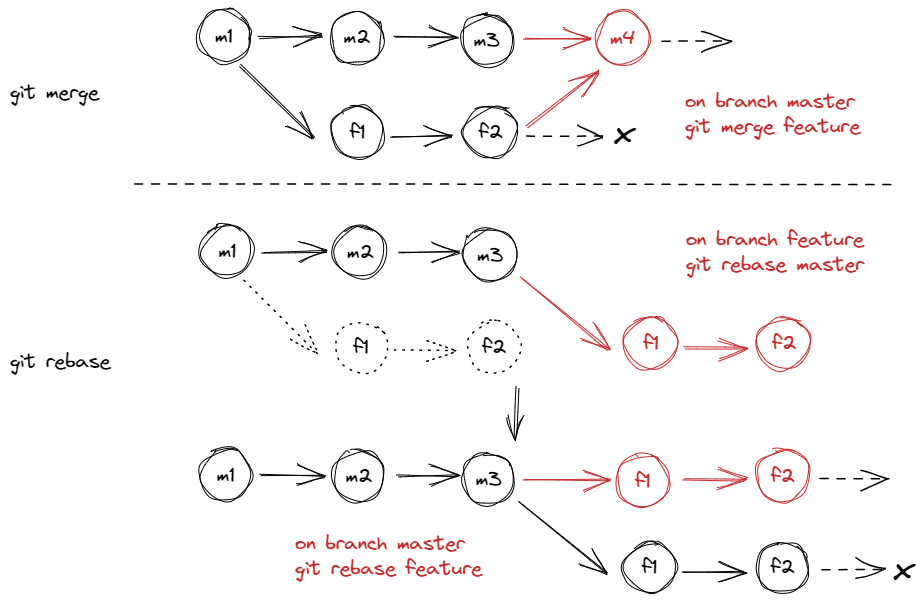
\includegraphics[width=350pt]{chapters/ch-software-management-advanced/figures/gitrebase.png}
	\caption{Two approaches of integrating branches, \texttt{git merge} VS \texttt{git rebase}.} \label{ch:sma:fig:gitrebase}
\end{figure}

\section{Remote Repository Management} \label{ch:sma:sec:rrm}

\textit{GitHub} is an internet hosting service for software development and sharing using \textit{Git}. A user can create, manage, share and co-develop remote repositories on \textit{GitHub}. Notice that \textit{GitHub} is not the only place to host remote repositories. Some alternatives include \textit{GitLab} and \textit{Gitee}. Using \textit{Git}, it is possible to build a remote repository hosting server at home on a regular computer. In this section, only \textit{GitHub} is considered.

An \textit{https} URL is associated with each remote repository on \textit{GitHub}, for example \textit{https://github.com/torvalds/linux.git} for Linux kernel. This URL can be used to download the remote repository to a local machine, or to link (synchronize) a local repository with that remote repository.

Consider the case where there is already a remote repository, either under the user's \textit{GitHub} account or from the community. To download a clone of an existing repository to the local machine, use
\begin{lstlisting}
$ git clone <repository URL> [<local directory>]
\end{lstlisting}
and to maintain the local repository up-to-date with the remote repository, regularly use
\begin{lstlisting}
$ git remote update
$ git pull
\end{lstlisting}
to synchronize the local repository with the remote one.

\begin{shortbox}
\Boxhead{Should I use \texttt{git pull}?}

One may argue whether it is a good idea to use \verb|git pull|. Although convenient, \verb|git pull| is an integration of two commands, \verb|git fetch| and \verb|git merge| (or \verb|git rebase|) executed sequentially. It may be ``safer'' to manually run the two commands separately.
\end{shortbox}

The local commits can also be pushed to the remote repository using
\begin{lstlisting}
$ git push
\end{lstlisting}
if the remote repository is under the user's account, or if the owner of the remote repository gives the user the permission. Notice that when pushing updates to the remote repository, \textit{GitHub} may require login credentials for permission checks.

Consider the case where there is already a local repository, and an empty repository has just been created on \textit{GitHub}. To setup the connection, navigate to the local repository and use
\begin{lstlisting}
$ git remote add <remote repository name> <repository URL>
\end{lstlisting}
which will register the remote repository URL in the local configuration file.

The next step is to map the local current working branch with a branch in the remote repository, which would be used as the default source/target branch when running \verb|git pull| and \verb|git push|. This can be done as follows.
\begin{lstlisting}
$ git branch --set-upstream-to <remote repository name> <remote repository branch>
\end{lstlisting}
Notice that this step is not required if the project is cloned from a remote repository using \verb|git clone| introduced earlier.

From there on, use \verb|git push| and \verb|git pull| normally.

Finally, to revert a commit that has already been pushed to a shared server, using \verb|git reset| in the local repository to erase the faulty commit, then \verb|git push| to push the erased repository to the remote repository would not work. This is because by erasing the latest commit locally, the local commit will be ``behind'' the remote repository, making \textit{Git} think that the local repository needs to be updated to follow the remote repository.

To tackle this problem, use \verb|git revert| instead as follows.
\begin{lstlisting}
$ git revert <commit ID>
\end{lstlisting}
Different from \verb|git reset|, this command creates a new commit that mirrors the specified historical commit. The new commit can then be pushed to the shared server.













